\begin{enumerate}
\item  Prove that the points $\myvec{3,0}, \myvec{6, 4}$ and $\myvec{-1, 3}$ are the vertices of a right angled isosceles triangle.\\
\item  If the point $P\myvec{x, y}$ is equidistant from the points $A\myvec{a+b, b-a}$ and $B\myvec{a-b, a+b}$. Prove that $bx=ay$.\\
\item In fig \ref{figure_1}, the vertices of $\triangle ABC$ are $A\myvec{4, 6}, B\myvec{1, 5}$and $C\myvec{7, 2}$. A line-segment $DE$ is drawn to intersect the sides $AB$ and $AC$ at $D$ and $E$ respectively such that $\dfrac{AD}{AB}$ = $\dfrac{AE}{AC}$ = $\dfrac{1}{3}$ . Calculate the area of $ \triangle ADE$ and compare it with area of $ \triangle ABC$.\\
	\begin{figure}[H]
      \centering
      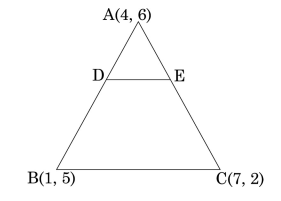
\includegraphics[width=5cm]{figs/2016_10_8.png}
     \caption{}
      \label{figure_1}
\end{figure} 
\item  Let $P$ and $Q$ be the points of trisection of the line segment joining the points $A\myvec{2,-2}$ and $B\myvec{-7, 4}$ such that $P$ is nearer to $A$. Find the coordinates of $P$ and $Q$.
\end{enumerate}
